\chapter{数据处理}
\label{chapter:dataprocess}

\section{特征工程}
\label{section:featEngineer}
\subsection{功能注释特征}
\label{subsection:GoSimilarity}

基因本体信息\cite{ashburner_gene_2000}即GO注释信息是描述蛋白质功能表达的词汇表,将生物活动过程进行统一编码表示,其在生物信息学邻域得到了广泛的应用。对应到蛋白质中,蛋白质分子参与的若干生物过程均可对应到GO注释表,形成对该蛋白质的综合功能描述。GO注释项总体分为三类,分别是生物过程(Biological Process)、分子功能(Molecular Function)及细胞组成(Cellular Component),生物过程描述分子功能有序组成的生命活动,分子功能描述分子在生物学上的活性,细胞组成描述了亚细胞结构及位置信息。GO注释项之间由于描述涵盖范围的不同,具有一定的从属关系,所有的GO注释项可以组成有向无环图(Directed Acyclic Graph,简称DAG)。图\ref{fig:go-dag}为QuickGO\cite{binns_quickgo_2009}网站中获取的生殖细胞发育过程对应的GO注释DAG图。GO注释信息的从属关系主要分为两种,分别是$is\_a$和$part\_of$,其中$is\_a$表示包含关系,如图中黑色箭头所示,$part\_of$表示从属关系,如图中蓝色箭头所示。图中每一个方框展示了GO注释项及其生物功能。

\begin{figure}[htbp]
    \centering
    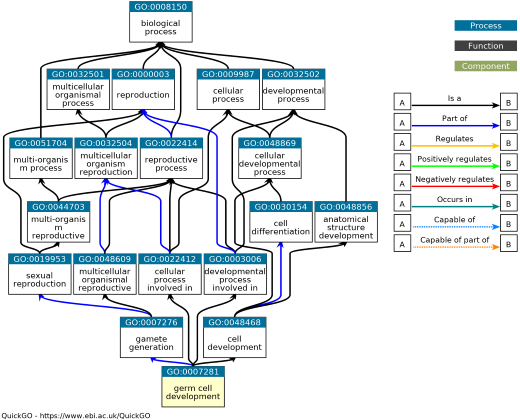
\includegraphics{go-dag}
    \caption{生殖细胞发育对应的GO示意图}
    \label{fig:go-dag}
\end{figure}

通常情况下,蛋白质复合物中蛋白质倾向于相同的功能表达,同时功能表达相似性越高时,蛋白质产生相互作用的可能性越大。部分算法\cite{ulitsky_identification_2007,jianxing_feng_max-flow-based_2011}基于功能表达数据提出了$PIN$连边权重更新的方法。
本文采用两种方法计算蛋白质功能相似度,将计算结果作为$PIN$网络中邻边的蛋白质功能特征。

第一种蛋白质功能相似度计算方法为Wang等人\cite{wang_new_2007}提出的方法。

给定一个GO注释项$p$,从GO的总体DAG图中提取子图$DAG_p(A,T_p,E_p)$,其中$T_p$是$p$及所有$p$的祖先结点的注释项,$E_p$表示所有截取的注释项的连接关系。
定义$T_p$中每一个结点对$p$的语义值如下:
\begin{equation}
    \label{equ:feat:go:SAT}
    S_p(t)=\left\{\begin{array}{l}
        1,t=p                                                                        \\
        \max {\{ w_e\times S_p(t^\prime )| t^\prime\in ~children~of~(t) \} },t\neq p \\
    \end{array}\right.
\end{equation}
其中$w_e$是$t^\prime$和$t$之间的权重,定义两种类型的边$is\_a$和$part\_of$权重各自为0.8和0.6。有公式可以直观得出,祖先结点点中离$p$注释越远的注释项,其对$p$的语义值越小,而$p$对自身的语义值贡献为1。
定义了所有祖先结点对$p$的语义值之后,可以直接得出$p$的语义值得分,计算公式如下:
\begin{equation}
    \label{equ:feat:go:SVA}
    SV(p)=\sum_{t \in T_p}(t)
\end{equation}
按照该计算方法,可以得到每一个注释项各自的语义值,在此基础上可以得到两个注释项$p$,$q$语义值的相似度,具体计算方法如下:
\begin{equation}
    \label{equ:feat:go:SimItemWang}
    WSim_{GO}(p,q)=\frac{\sum_{t \in T_p \cap T_q}(S_p(t)+S_q(t))}{SV(p)+SV(q)}
\end{equation}
其中$t$为$p$和$q$的所有公共祖先结点。由于蛋白质通常是由多个注释项组成,因此蛋白质之间的功能相似性需要考虑两个蛋白质各自注释项之间的综合结果,其具体计算方法如下:
\begin{equation}
    \label{equ:feat:go:SimProteinWang}
    \begin{aligned}
        WSim_{Protein}(P,Q) & =\frac{1}{m+n}\cdot \left\{\sum_{1\leq i\leq m}{\max_{1\leq j\leq n}[{Sim_{GO}(p_i,q_j)}}]\right. \\
                            & \left.+\sum_{1\leq j\leq n}{\max_{1\leq i\leq m}[{Sim_{GO}(p_i,q_j)}}]\right\}
    \end{aligned}
\end{equation}
其中$P$,$Q$表示两个蛋白质,其中分别具有$\{p_i| i=1,2,\dots,m\}$,$\{q_j| j=1,2,\dots,n\}$的功能注释项。
这个方法的核心思想是将两个蛋白质的注释信息相互关系矩阵$m\times n$构造出来,只考虑源蛋白质的某一个注释项和目标蛋白质所有注释项最大的相关性,而蛋白质的相互作用关系是所有最大值的平均。

第二种蛋白质功能相似度计算方法为Lin等人\cite{lin_information-theoretic_1998}提出的方法。首先计算某两个注释项之间的相关性,具体计算过程如下:
\begin{equation}
    \label{equ:feat:go:SimItemLin}
    LSim_{GO}(p,q)=\min_{anc \in Ancient(p,q)}\mathcal{P} (anc)
    % Sim_{GO}(p,q)=\max{\frac{2\times \log }{} }
\end{equation}
其中$Ancient(p,q)$表示两个注释项的公共祖先,而$\mathcal{P}$表示某一个注释项在所有蛋白质中出现的概率。这个计算公式直观的认为,两个具有相互关联的功能注释,其关联结点越稀有,则表示两个注释项的相关性越强。计算蛋白质功能相似性的计算方法如下:
\begin{equation}
    \label{equ:feat:go:SimProteinLin}
    LSim_{Protein}(P,Q)=\max{\frac{2\times \log \{Sim_{GO}(p,q)\}}{\log {\mathcal{P}_p}+\log {\mathcal{P}_q}} }
\end{equation}


\subsection{结构域特征}
\label{subsection:domainSimilarity}
蛋白质结构域时蛋白质具有独立功能和特异结构的区域,结构域互作信息影响蛋白质复合物的形成\cite{kim_relating_2006}。结构域之间具有相互作用关系,这些相互作用关系可以从三维交互域(3did)数据库\cite{mosca_3did_2014}提取,并构建成结构域相互作用网络(Domain-Domain Interaction Network,简称DDI)。
单个蛋白质所具有的结构域可以映射到结构域互作网络的若干结点,成为一个结构域集群,而蛋白质域相似性可以转换为两个结构域集群的相互作用关系。
本文中两个蛋白质的结构域互作特征包括如下方面:两个蛋白质结构域交集、并集以及相互之间的差集;映射到结构域相互网络之后,两个结构域集群之间的相互作用关系数量,其具体的计算公式如下:
\begin{equation}
    \label{equ:feat:domain}
    Sim_{domain} = \sum_{i \in dom(p)}{\sum_{j \in dom(q)}{Weight_{ij}}}
\end{equation}
其中$i$、$j$分别时蛋白质$p$、$q$之间的结构域,$Weight_{ij}$代表结构域$i$、$j$在结构域相互作用网络中的作用强度,对于无权网络可以取值为1。

huang等人\cite{huang_protein-protein_2013}在运用结构域相互作用网络预测蛋白质相互作用时,提出了使用一阶邻居和二阶邻居计算$domain$相似性的想法,其扩展方式如图\ref{fig:domain-second}所示。本文也同时补充了一阶和二阶扩展之后的蛋白质$domain$相似性特征。
\begin{figure}[htbp]
    \centering
    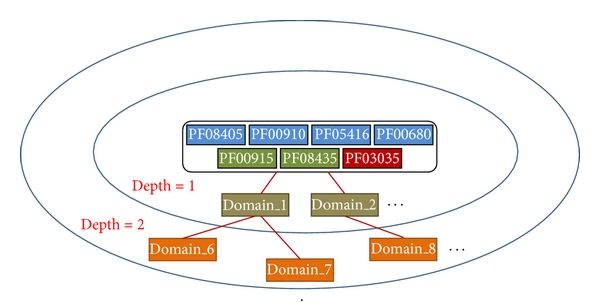
\includegraphics{domain-second}
    \caption{DDI多阶邻居示意图}
    \label{fig:domain-second}
\end{figure}


\subsection{亚细胞定位特征}
\label{subsection:SubcellSimilarity}
细胞是一个高度有序的结构,胞内根据空间分布和功能不同,可以分成不同细胞器或细胞区域,蛋白质只有转运到正确的部位才能参与细胞的各种生命活动,ZHANG等人\cite{zhang_protein_2007}认为蛋白质的亚细胞定位有助于研究蛋白质的生物学功能,同时对蛋白质的其他研究如相互作用、进化等也能提供必要的信息。huang等人提出\cite{fan_genome-wide_2017}使用蛋白质复合物和亚细胞定位信息预测关键蛋白质,蛋白质复合物,蛋白质复合物的生成和功能实现和其所处的细胞位置相关,因此蛋白质的亚细胞定位能对蛋白质复合物的形成产生一定的影响。本文将两个蛋白质亚细胞定位数据的交集和并集作为蛋白质的亚细胞定位特征。图\ref{fig:subcell}为苏氨酸蛋白激酶TOR1亚细胞定位图,其中黄色的部分表示其主要的注释区域,包括细胞膜和液膜。

\begin{figure}[htbp]
    \centering
    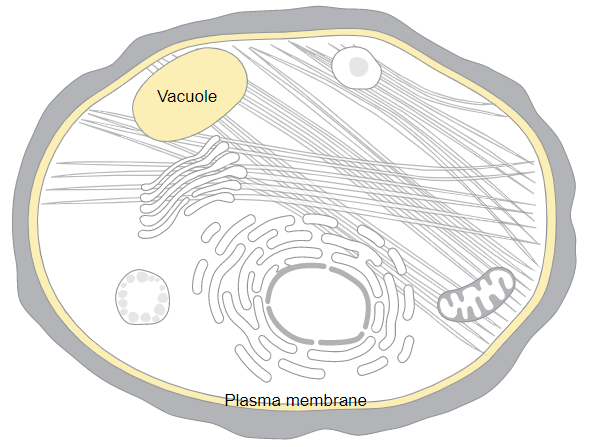
\includegraphics{subcell}
    \caption{苏氨酸蛋白激酶TOR1亚细胞定位图}
    \label{fig:subcell}
\end{figure}

\subsection{拓扑相似性特征}
\label{subsection:TopoSimilarity}
蛋白质在$PIN$中所处的拓扑环境也可以作为蛋白质相似性特征的计算方式。惭愧DPClus算法\cite{altaf-ul-amin_development_2006},本文将结点的公共邻居数作为拓扑相似性特征。具体计算方法如下:
\begin{equation}
    \label{equ:feat:topoCN}
    CN_{(P,Q)} = \left\lvert N_P\cap N_Q\right\rvert
\end{equation}
其中$P$,$Q$为相互作用的蛋白质,$N_P$和$N_Q$分别为两个蛋白质在$PIN$中的邻居。

\subsection{数据处理阶段特征汇总}
\label{subsection:SimSummary}
在数据预处理阶段,本文计算了$PIN$中所有蛋白质相互作用之间的相似性特征,其中包括蛋白质功能注释特征、结构域特征、亚细胞定位特征以及网络拓扑特征。$PIN$中每条相互作用边所具有的特征维度为12维,具体分布如表\ref{tab:PINedgeFeatNUms}所示:
\begin{table}[h]
    \centering
    \caption{$PIN$边特征维度分布}
    \label{tab:PINedgeFeatNUms}
    \begin{tabular}{C{3cm}C{3cm}C{3cm}C{3cm}}
        \toprule
        \textbf{功能注释特征} & \textbf{结构域特征} & \textbf{亚细胞定位特征} & \textbf{网络拓扑特征} \\
        \midrule
        2                     & 7                   & 2                       & 1                     \\
        \bottomrule
    \end{tabular}
\end{table}


\section{网络结构构建}
\label{section:NetConstruc}
由于酿酒酵母(Saccharomyces cerevisiae)的蛋白质相互作用中有较深入的研究,其标准复合物数据集,蛋白质相互作用数据较为完备,因此本文基于酿酒酵母的网络展开研究。

本文选取了主流的酿酒酵母细菌的$PPI$数据集,包括DIP\cite{salwinski_database_2004}、Krogan\cite{krogan_global_2006}、Biogrid\cite{stark_biogrid_2006}和Gavin\cite{gavin_proteome_2006}。

DIP数据集是结合各种来源的信息创建的一致的$PPI$数据集,可以自动从论文中提取关系数据并更新数据库,同时有专业人员管理。
Krogan数据集使用$LC_MS/MS$技术检测蛋白质相互作用并借助机器学习方法提高结果的可靠度,数据集分为核心和附属两个部分,本文将核心附属网络融合进行实验。
Biogrid数据集融合了多个数据集来源,同时排出了不符合多重验证标准的相互作用。
Gavin数据集基于亲和纯化与质谱技术检测蛋白质相互作用,并使用socio-affinity指数评估$PPI$检测结果的可靠度。

每个数据集都由若干蛋白质相互作用对组成,表示两个蛋白质之间存在相互作用关系,依据关系数据,可以相应的构造$PIN$。数据集具体的网络结构如图\ref{fig:ppi-datasets}所示,具体统计学特征如表\ref{tab:PPIStatic}所示。

\begin{figure}[htbp]
    \centering
    \subcaptionbox{DIP数据集}{\label{fig:ppi:zitu:a}
        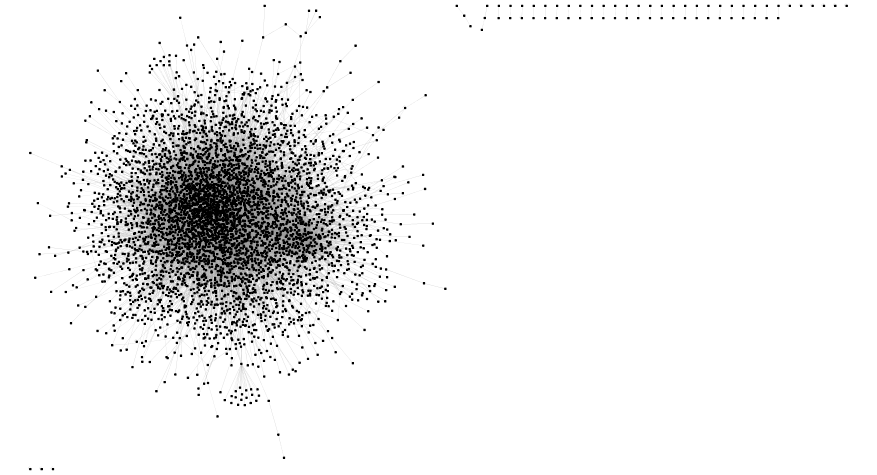
\includegraphics[width=9cm]{ppi-dip}}
    \vskip0.5cm
    \subcaptionbox{Krogan数据集}{\label{fig:ppi:zitu:b}
        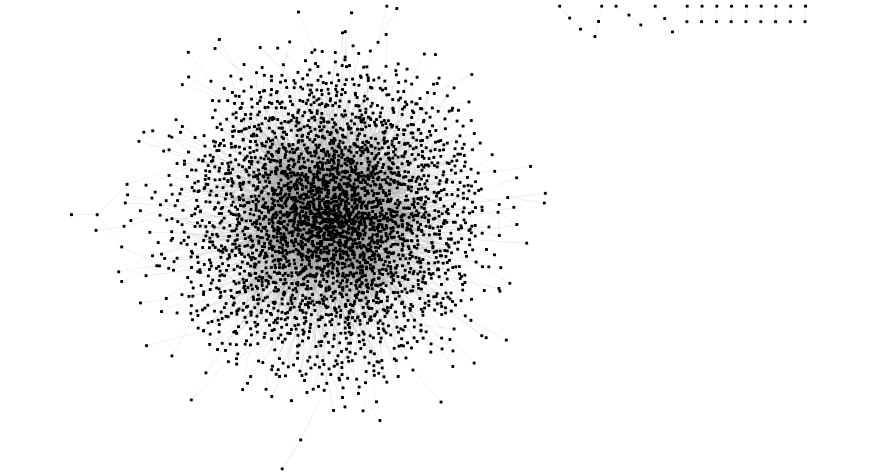
\includegraphics[width=9cm]{ppi-krogan}}
    \vskip0.5cm
    \subcaptionbox{biogrid数据集}{\label{fig:ppi:zitu:c}
        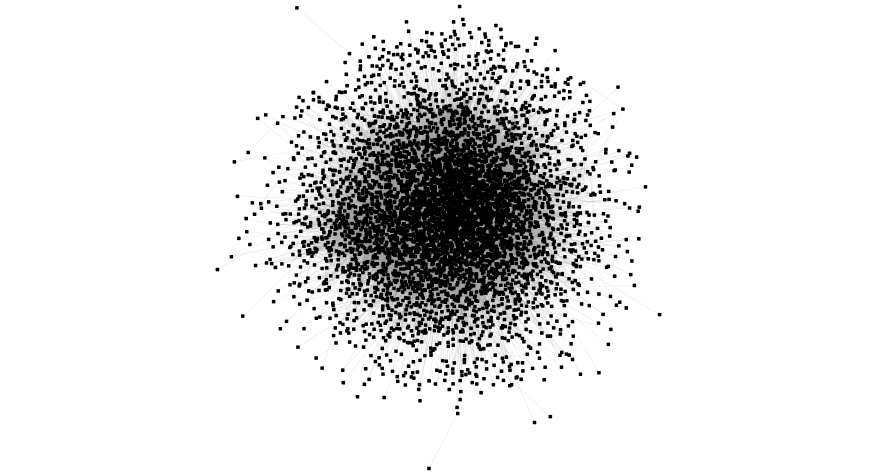
\includegraphics[width=9cm]{ppi-biogrid}}
    \vskip0.5cm
    \subcaptionbox{Gavin数据集}{\label{fig:ppi:zitu:d}
        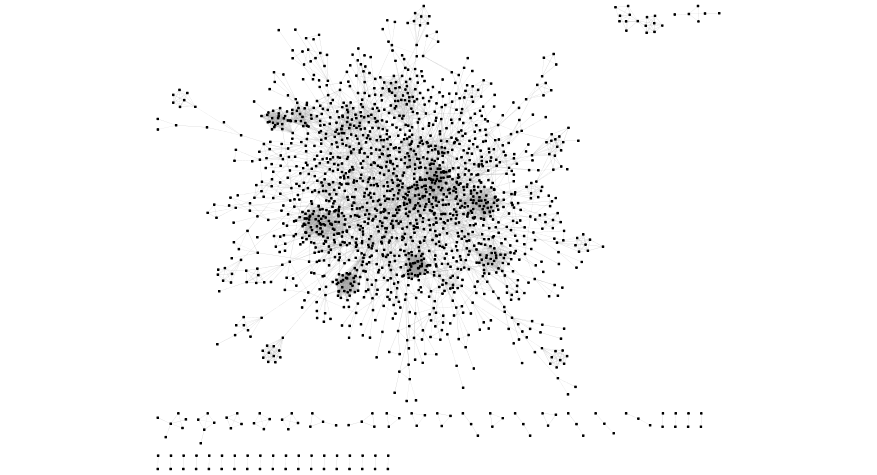
\includegraphics[width=9cm]{ppi-gavin}}
    \caption{蛋白质相互作用数据集}
    \label{fig:ppi-datasets}
\end{figure}


\begin{table}[h]
    \centering
    \caption{$PPI$数据集统计表}
    \label{tab:PPIStatic}
    \begin{tabular}{L{4.2cm}L{2cm}L{2cm}L{2cm}L{2cm}}
        \toprule
        \textbf{网络特征} & \textbf{DIP} & \textbf{Krogan} & \textbf{Biogrid} & \textbf{Gavin} \\
        \midrule
        蛋白质数          & 4928         & 3672            & 5573             & 1855           \\
        相互作用数        & 17201        & 14317           & 59636            & 7669           \\
        平均度数          & 6.98         & 7.80            & 21.40            & 8.27           \\
        密度              & 0.0014       & 0.0021          & 0.0038           & 0.0044         \\
        平均聚类系数      & 0.0945       & 0.1203          & 0.2483           & 0.4674         \\
        连通个数          & 28           & 14              & 1                & 43             \\
        最大连通结点数    & 4873         & 3642            & 5573             & 1727           \\
        传递性            & 0.0728       & 0.1001          & 0.0657           & 0.5676         \\
        直径              & 11           & 10              & 6                & 13             \\
        \bottomrule
    \end{tabular}
\end{table}

从表\ref{tab:PPIStatic}中可以看出,DIP数据集和Biogrid数据集是结点数和邻边数最大的两个数据集,同时其度数差异性较大,本文的研究工作主要围绕这两个数据集展开。最后,模型效果也会在Krogan数据集和Gavin数据集进行验证。

利用$PPI$数据集构建相应的$PIN$网络结构之后,可以将蛋白质特征以及蛋白质相互作用特征添加到网络中去,形成带有生物特征的蛋白质相互作用网络$Feated-PIN$。在结点上添加蛋白质自有的特征,比如蛋白质序列长度、分子重量等等,以此作为结点的初始特征,同时在邻边上添加通过生物计算的蛋白质相互作用特征,作为图网络里面邻边的初始特征。

\section{数据集提取与划分}
\label{section:datasetExtract}
在$Feated-PIN$的基础上,按照复合物的对应结点抽取局部图$Feated-subGraph$,该局部图包含了复合物内部蛋白质之间的相互作用关系、相关性特征数据及部分蛋白质特征数据,因此可以将局部图作为后续复合物筛选模型的输入数据。

本文正样本由酵母菌标准复合物数据集CYC2008\cite{pu_up--date_2009}和MIPS\cite{pagel_mips_2005}构成,负样本为$PIN$上在一定限制条件下产生的随机子图。COACH算法\cite{leung_predicting_2009}作为在复合物预测方法中具有一定准确度和鲁棒性的方法,其产生的样本作为中间样本。

\subsection{标准复合物子图数据}
\label{subsection:standardComplex}
本文融合了CYC2008和MIPS数据集,剔除了其中邻居相似性(公式\ref{equ:compComplexSim:NA})过高的部分,剩余的样本数为734。
在PPI网络中,可能存在部分结点缺失,为了保证标准复合物的准确性,在训练过程中我们舍弃具有缺失的标准复合物。具体数据为在Biogrid网络中,正样本个数为621个,在DIP网络中,正样本个数为371。
\subsection{中间样本复合物子图数据}
\label{subsection:middleComplex}
中间样本由无权COACH算法运行在目标网络中产生,需要对标准复合物和随机复合物具有一定的区分度,同时能对分类器识别复合物具有指导作用。一般情况下,通常复合物预测算法无法无法得到和标准集中的复合物完全相同的结果,在邻居相似性大于0.25时就认为复合物预测成功。

依据基于邻居相似性的分类标准,COACH生成的样本中有部分复合物预测成功,剩余的复合物预测失败,本文对分类模型的要求时可以区分这两类样本。在可区分该两类样本的情况下,模型对其他算法产生的结果进行筛选时,才可以正确的定位到其中预测成功的样本。因此本文将COACH生成的样本分为两类。
由于邻居相似性处于0.25附近时,样本可能具有较大的迷惑性,反而影响模型的正常训练,因此剔除相似性在0.25附近的部分样本。

本文对中间样本具体做如下处理:
\begin{enumerate}
    \item 计算各个样本和标准复合物的最高邻居相似性,得到0$\thicksim$1的分数;
    \item 剔除其中相似性分数高于0.8的样本,防止样本与标准集重合;
    \item 将相似性分数在0.4$\thicksim$1的样本作为A样本;
    \item 将相似性分数在0$\thicksim$0.2的样本作为B样本;
\end{enumerate}

经过上述处理,分别得到Biogrid网络和DIP网络运行COACH算法的中间样本数据集,其中Biogrid的A样本为192个、B样本为975个,DIP的A样本为179个、B样本为345个。
\subsection{随机复合物子图数据}
\label{subsection:randomComplex}

随机符合物是在互作网络中随机游走产生的随机图,结合标准样本和中间样本具有紧密型子图的特点,本文对随机游走算法做了一定限制。

首先按照图结点的权重选取初始结点,视作子图。对子图周围所有邻居结点设置权重,邻居结点与子图连接数越高,则该邻居结点权重越高。按照邻居结点权重加权随机抽取下一个结点,并将该结点加入子图,如此反复进行直至子图结点个数达到阈值。按照该种随机子图生成方法,子图趋向于密集连接。由于负样本在子图结构上和正样本相近,在进行分类任务时,可以避免模型学习简单的拓扑差异,迫使模型学习复合物内在的形成规律,达到主动学习的目的。图\ref{fig:diffrent-random-garphs}在DIP网络中采用不同随机算法得到的随机子图差异。

\begin{figure}[htbp]
    \centering
    \subcaptionbox{完全随机子图示意图1}{\label{fig:randomgraph:zitu:a}
        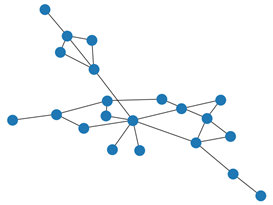
\includegraphics[width=5cm]{randomgraph-old-1}\hskip2cm}
    \subcaptionbox{完全随机子图示意图2}{\label{fig:randomgraph:zitu:b}
        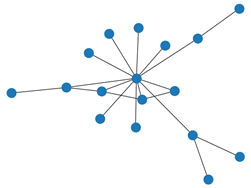
\includegraphics[width=5cm]{randomgraph-old-2}}
    \vskip0.5cm
    \subcaptionbox{限制性随机子图示意图1}{\label{fig:randomgraph:zitu:c}
        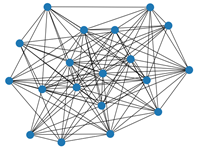
\includegraphics[width=5cm]{randomgraph-new-1}\hskip2cm}
    \subcaptionbox{限制性随机子图示意图2}{\label{fig:randomgraph:zitu:d}
        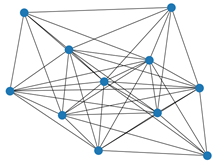
\includegraphics[width=5cm]{randomgraph-new-2}}
    \caption{不同随机算法获取的负样本差异图}
    \label{fig:diffrent-random-garphs}
\end{figure}


本文在网络中按照真实样本的结点数分布抽取负样本,负样本个数为标准样本和中间样本之和。

\subsection{总体数据集}
\label{subsection:allComplex}
最终产生的整体结果如下表所示:

\begin{table}[h]
    \centering
    \caption{数据集分布统计表}
    \label{tab:datasets:statistic}
    \begin{tabular}{C{3cm}C{2cm}C{3cm}C{3cm}C{2cm}}
        \toprule
        \textbf{网络} & \textbf{正样本数} & \textbf{中间样本数(A)} & \textbf{中间样本数(B)} & \textbf{负样本数} \\
        \midrule
        Krogan数据集  & 621               & 192                      & 975                      & 819               \\
        DIP数据集     & 371               & 179                      & 345                      & 764               \\
        \bottomrule
    \end{tabular}
\end{table}

